\subsection*{Modello 2 - small-1202 e small-1203}

% Introduzione su strategia del training -> qual è l'obiettivo dell'esperimento?
Avendo sperimentato con i vari modelli, abbiamo iniziato a effettuare alcuni addestramenti aumentando il
numero di epoche. Si è deciso quindi di procedere con il training su tutti i parametri della rete e non
congelare alcuni layer con l'opzione \verb|freeze| ma bilanciando l'operazione optando per la dimensione
del modello più piccola quale la versione small YOLOv8s. 

Il numero di epoche per esecuzione è stato impostato a 120 e per tale motivo i vari modelli sono stati
nominati come \verb|small-120x|. Il primo dei due modelli, \verb|small-1202|, ha visto una esecuzione 
comunque non ottimale visto che alcuni dei valori di loss rispetto alla validazione non sono stati 
salvati per alcuni problemi durante l'esecuzione su colab. Ciononostante si è visto, come in figura
\ref*{fig:v2-1}, che i valori delle funzioni di loss continuavano a decrescere mentre le metriche
o rimanevano costanti, come precision e recall, o andavano a migliorare, come mAP50.

\begin{figure}[h]
    \centering
    \includegraphics[width=0.8\textwidth]{v_2/small-1202/results.png}
    \caption{Andamento funzioni di loss e metriche durante l'esecuzione di small-1202}
    \label{fig:v2-1}
\end{figure}

La fase di training è stata pertanto ripetuta con l'esecuzione \verb|small-1203| che rispetto al nome assegnatogli
ha avuto 300 epoche a disposizione per l'addestramento mantenendo gli stessi iperparametri del tentativo precedente.

% Dettagli configurazione, tipologia modello e iperparametri, dove è stato eseguito il train
Di seguito sono riportati tutti gli iperparametri più importanti che caratterizzano questi addestramenti:
%TODO aggiungere tabella iperparametri
-> aggiunto dropout


% Risultati training
    % - andamento training

    \begin{figure}[h]
        \centering
        \includegraphics[width=0.8\textwidth]{v_2/small-1203/results.png}
        \caption{Andamento funzioni di loss e metriche durante l'esecuzione di v8m12}
        \label{fig:v2-2}
    \end{figure}
    % - grafici recall e precision e performance e F1
    \begin{figure}[h]
        \centering
        \begin{subfigure}{.5\textwidth}
            \centering
            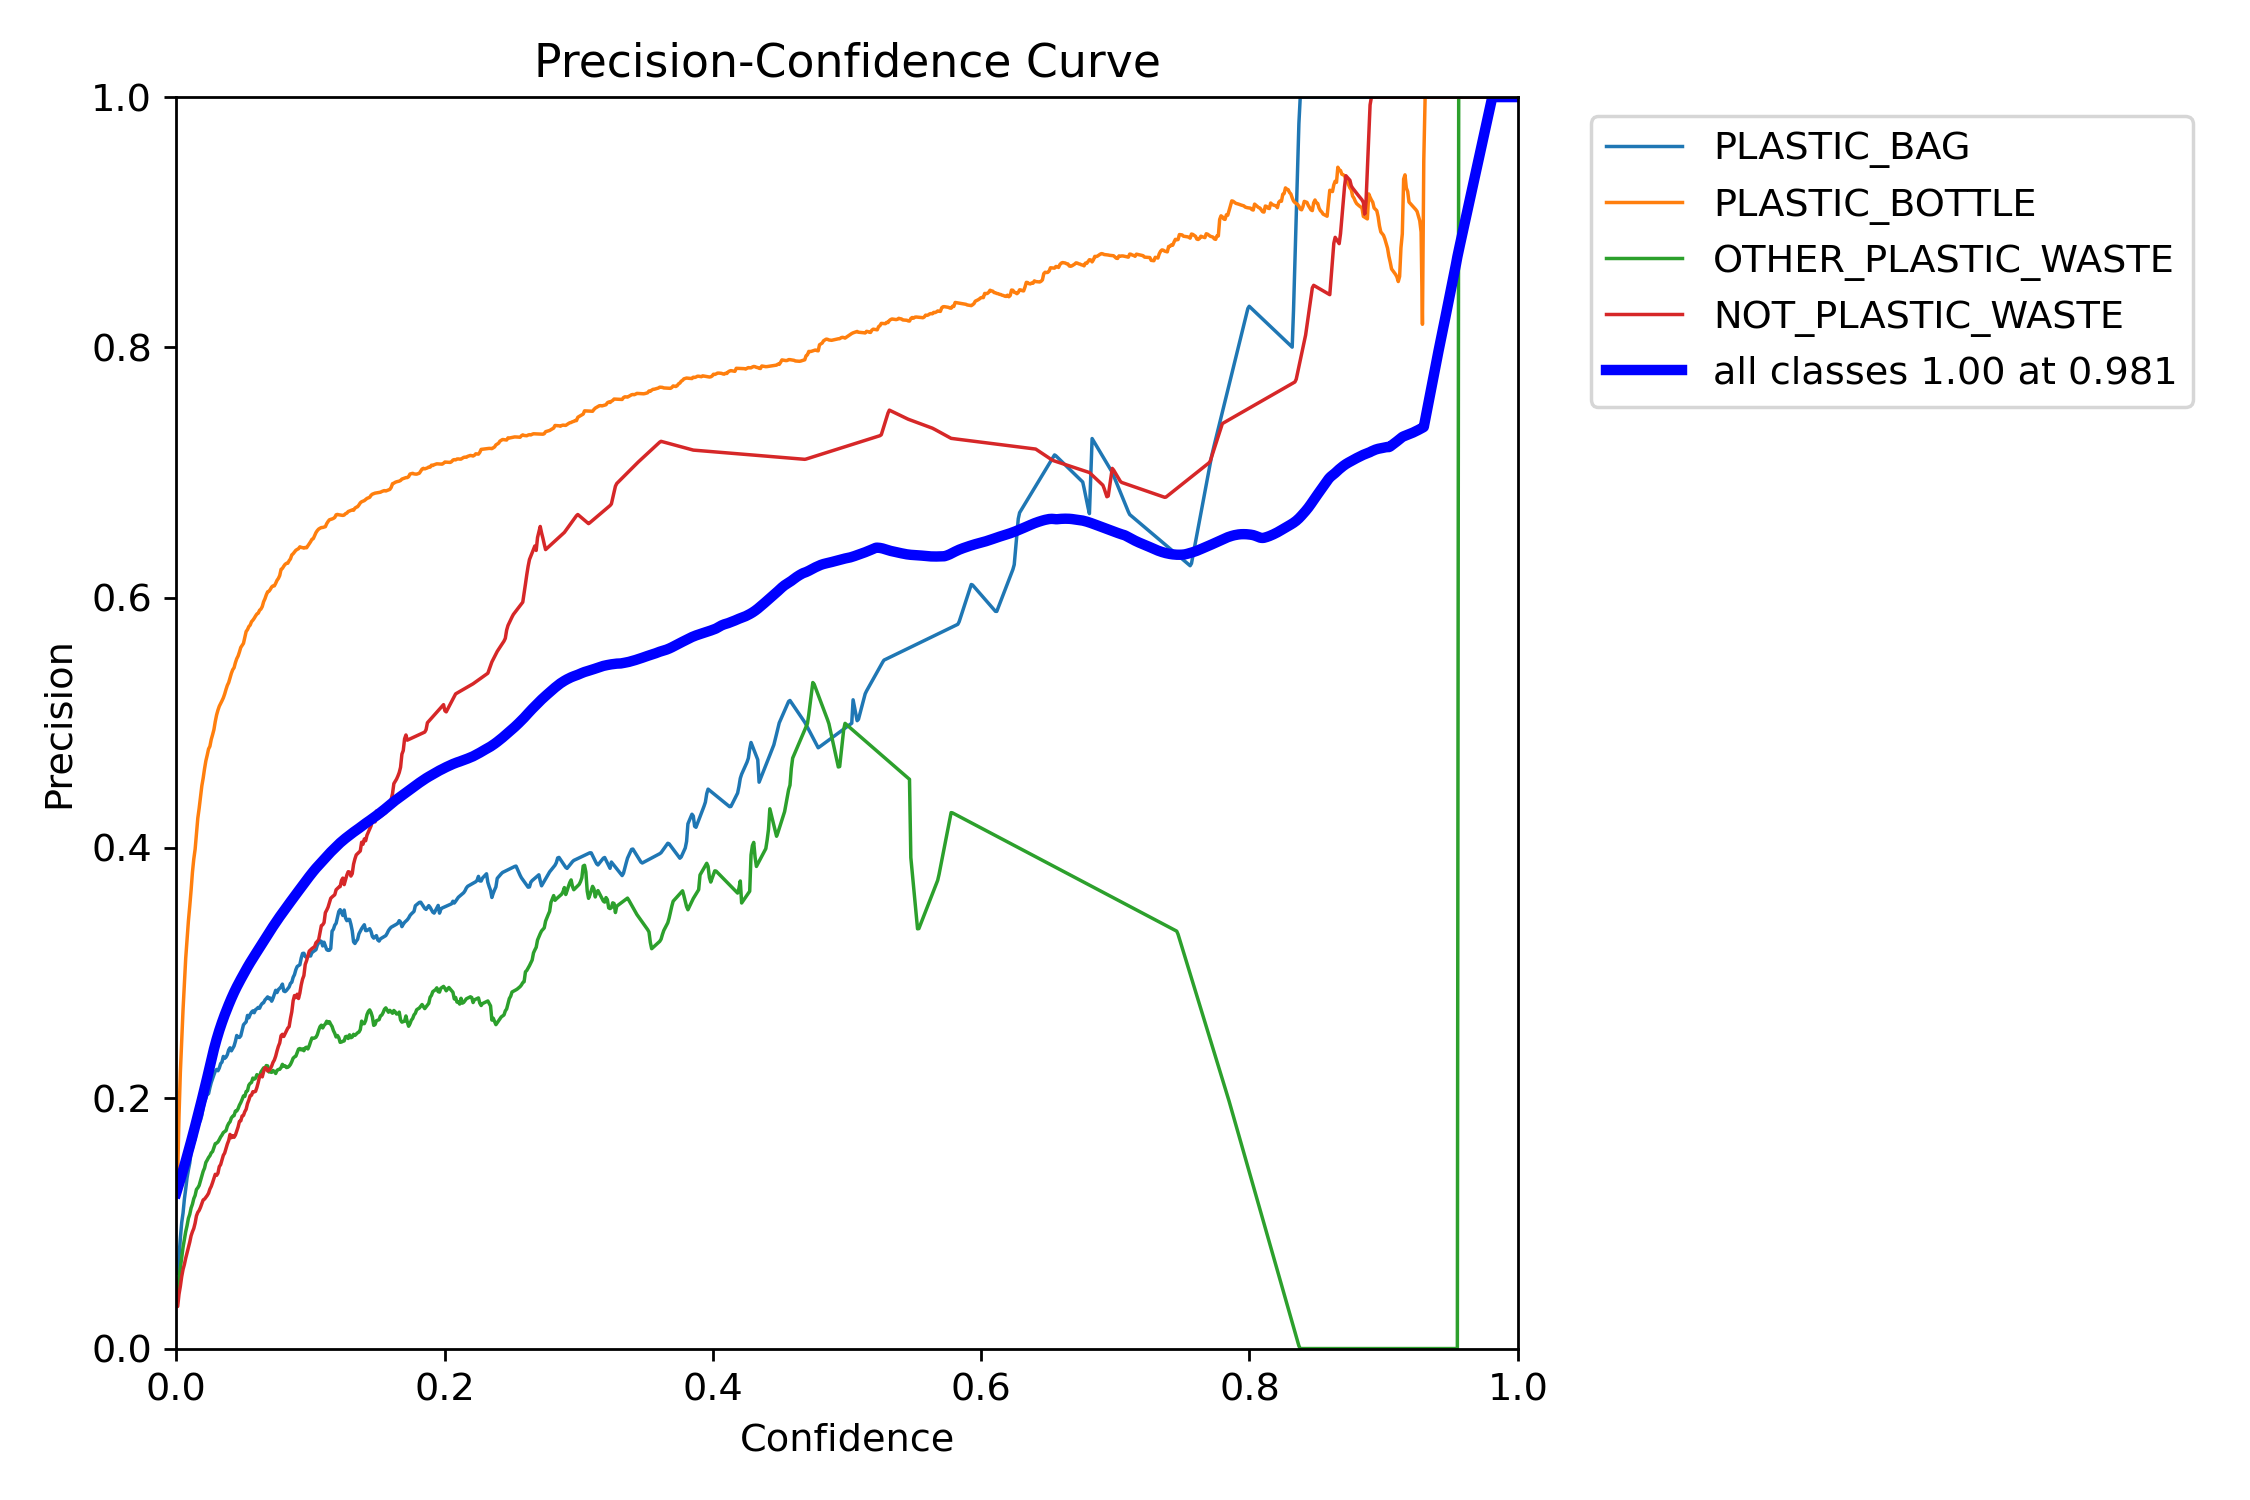
\includegraphics[width=.9\linewidth]{v_2/small-1203/P_curve.png}
            
            \label{fig:v2-3.1}
          \end{subfigure}%
          \begin{subfigure}{.5\textwidth}
            \centering
            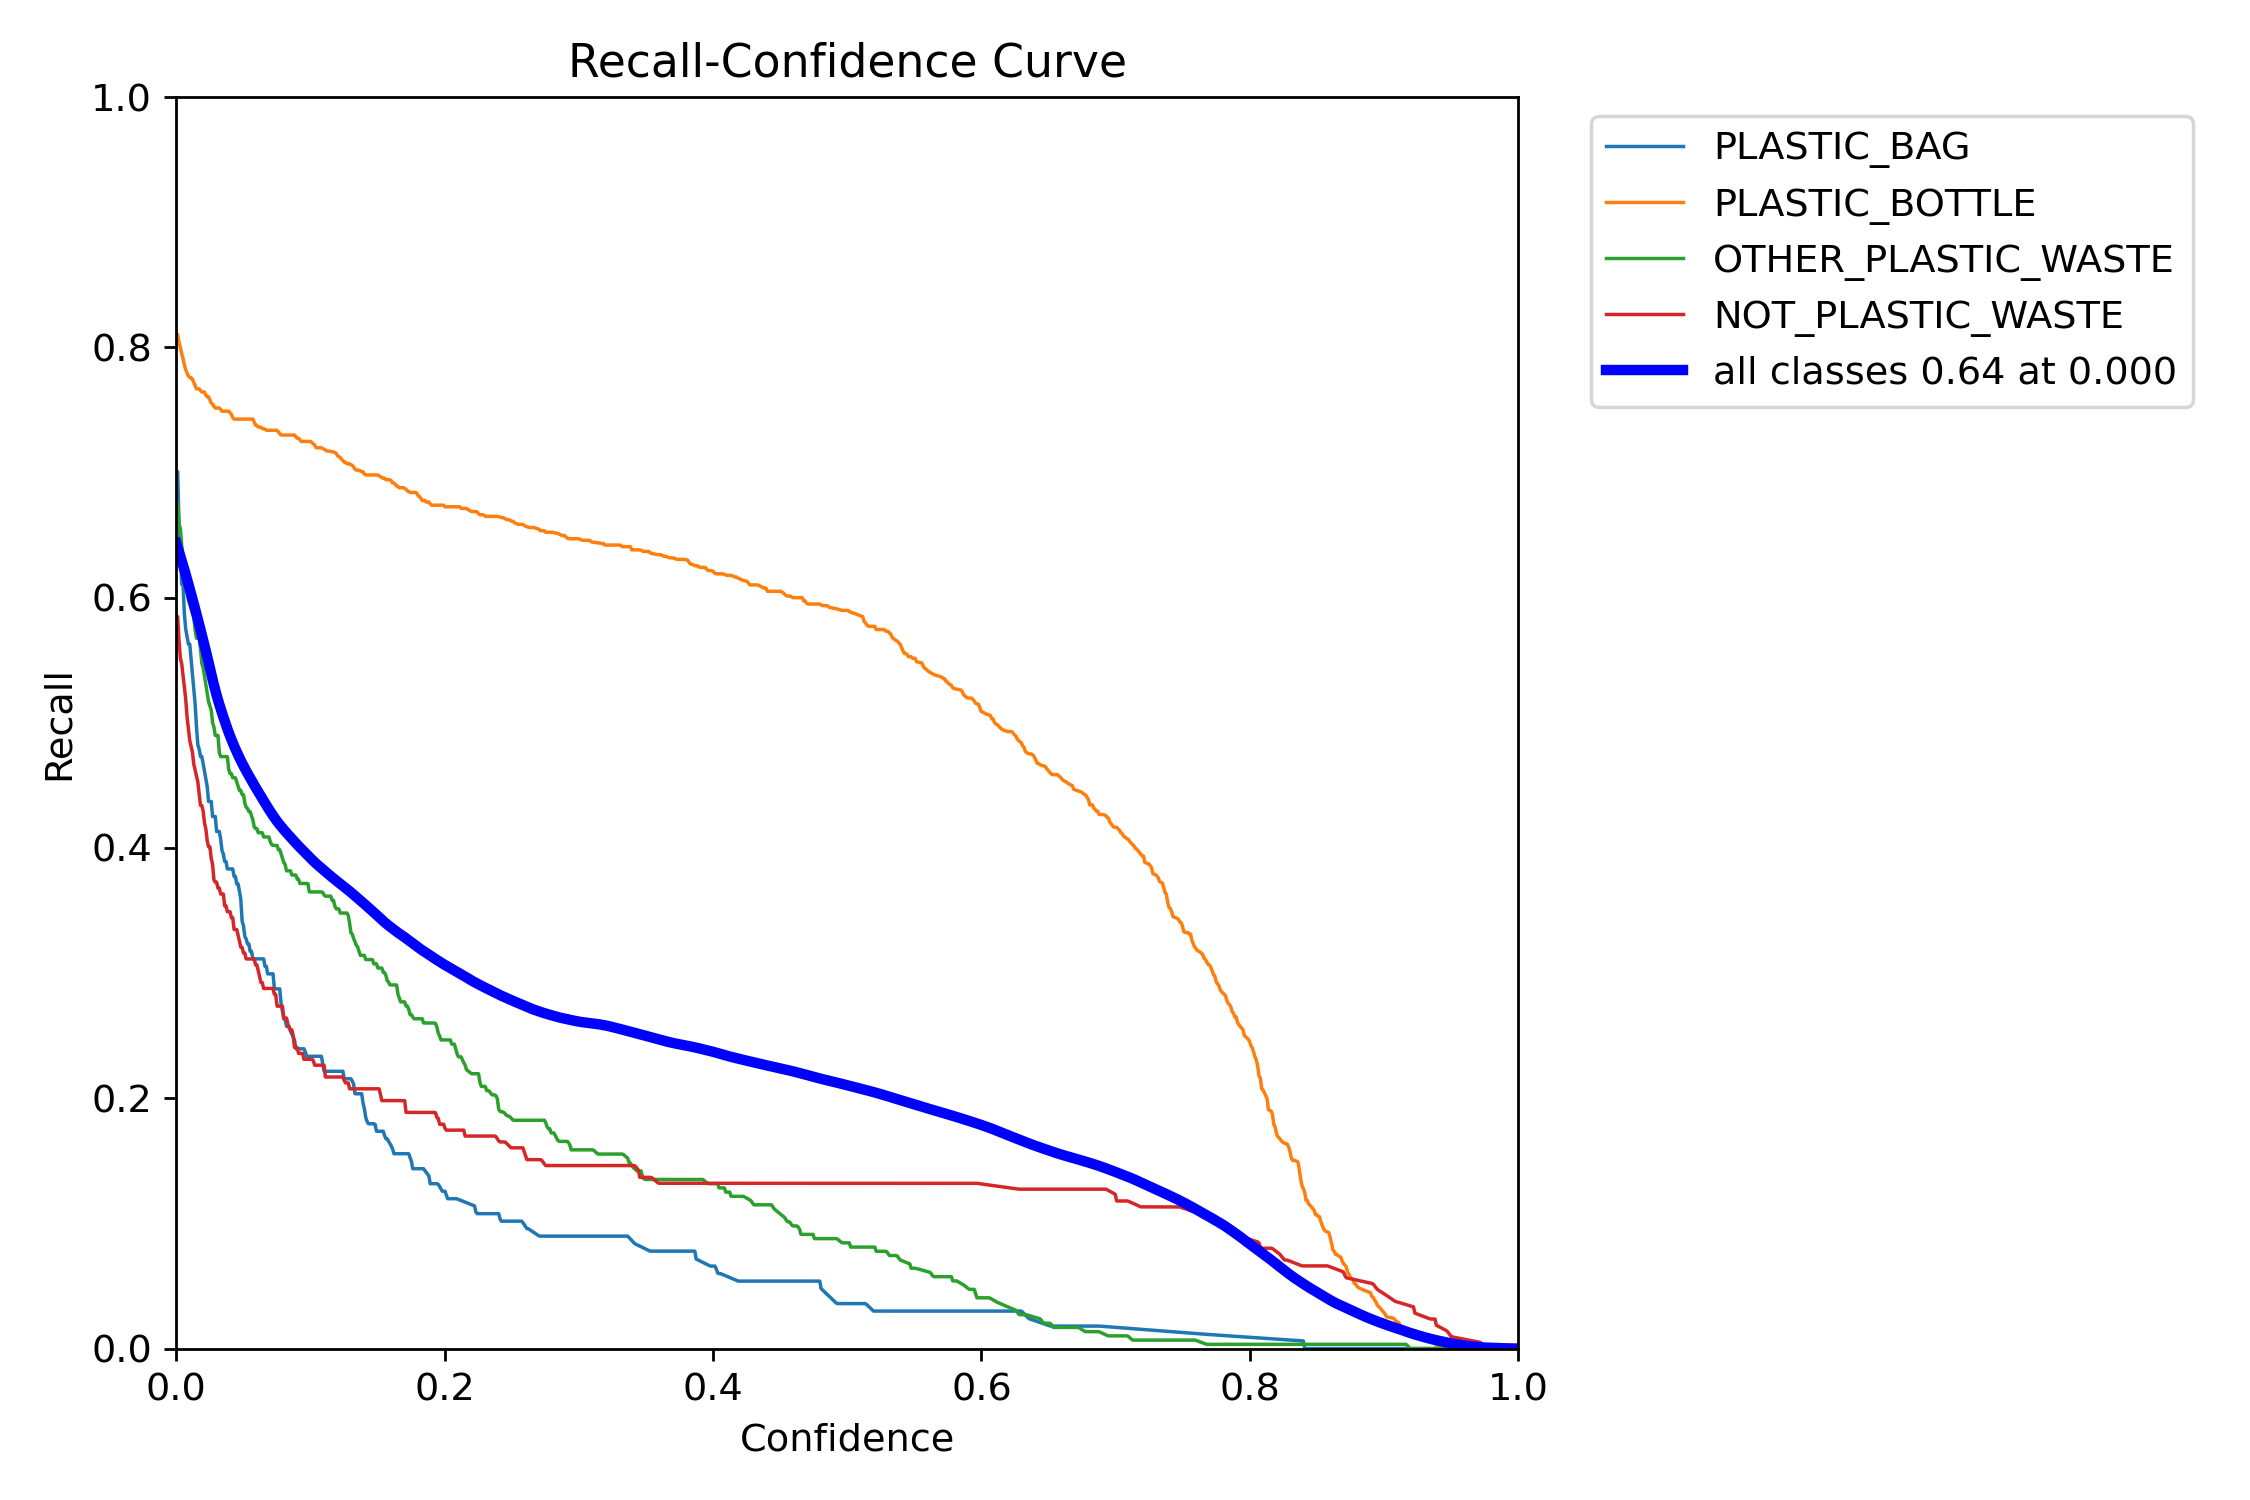
\includegraphics[width=.9\linewidth]{v_2/small-1203/R_curve.png}
            
            \label{fig:v2-3.2}
          \end{subfigure}
          \vskip\baselineskip
        \begin{subfigure}{.5\textwidth}
          \centering
          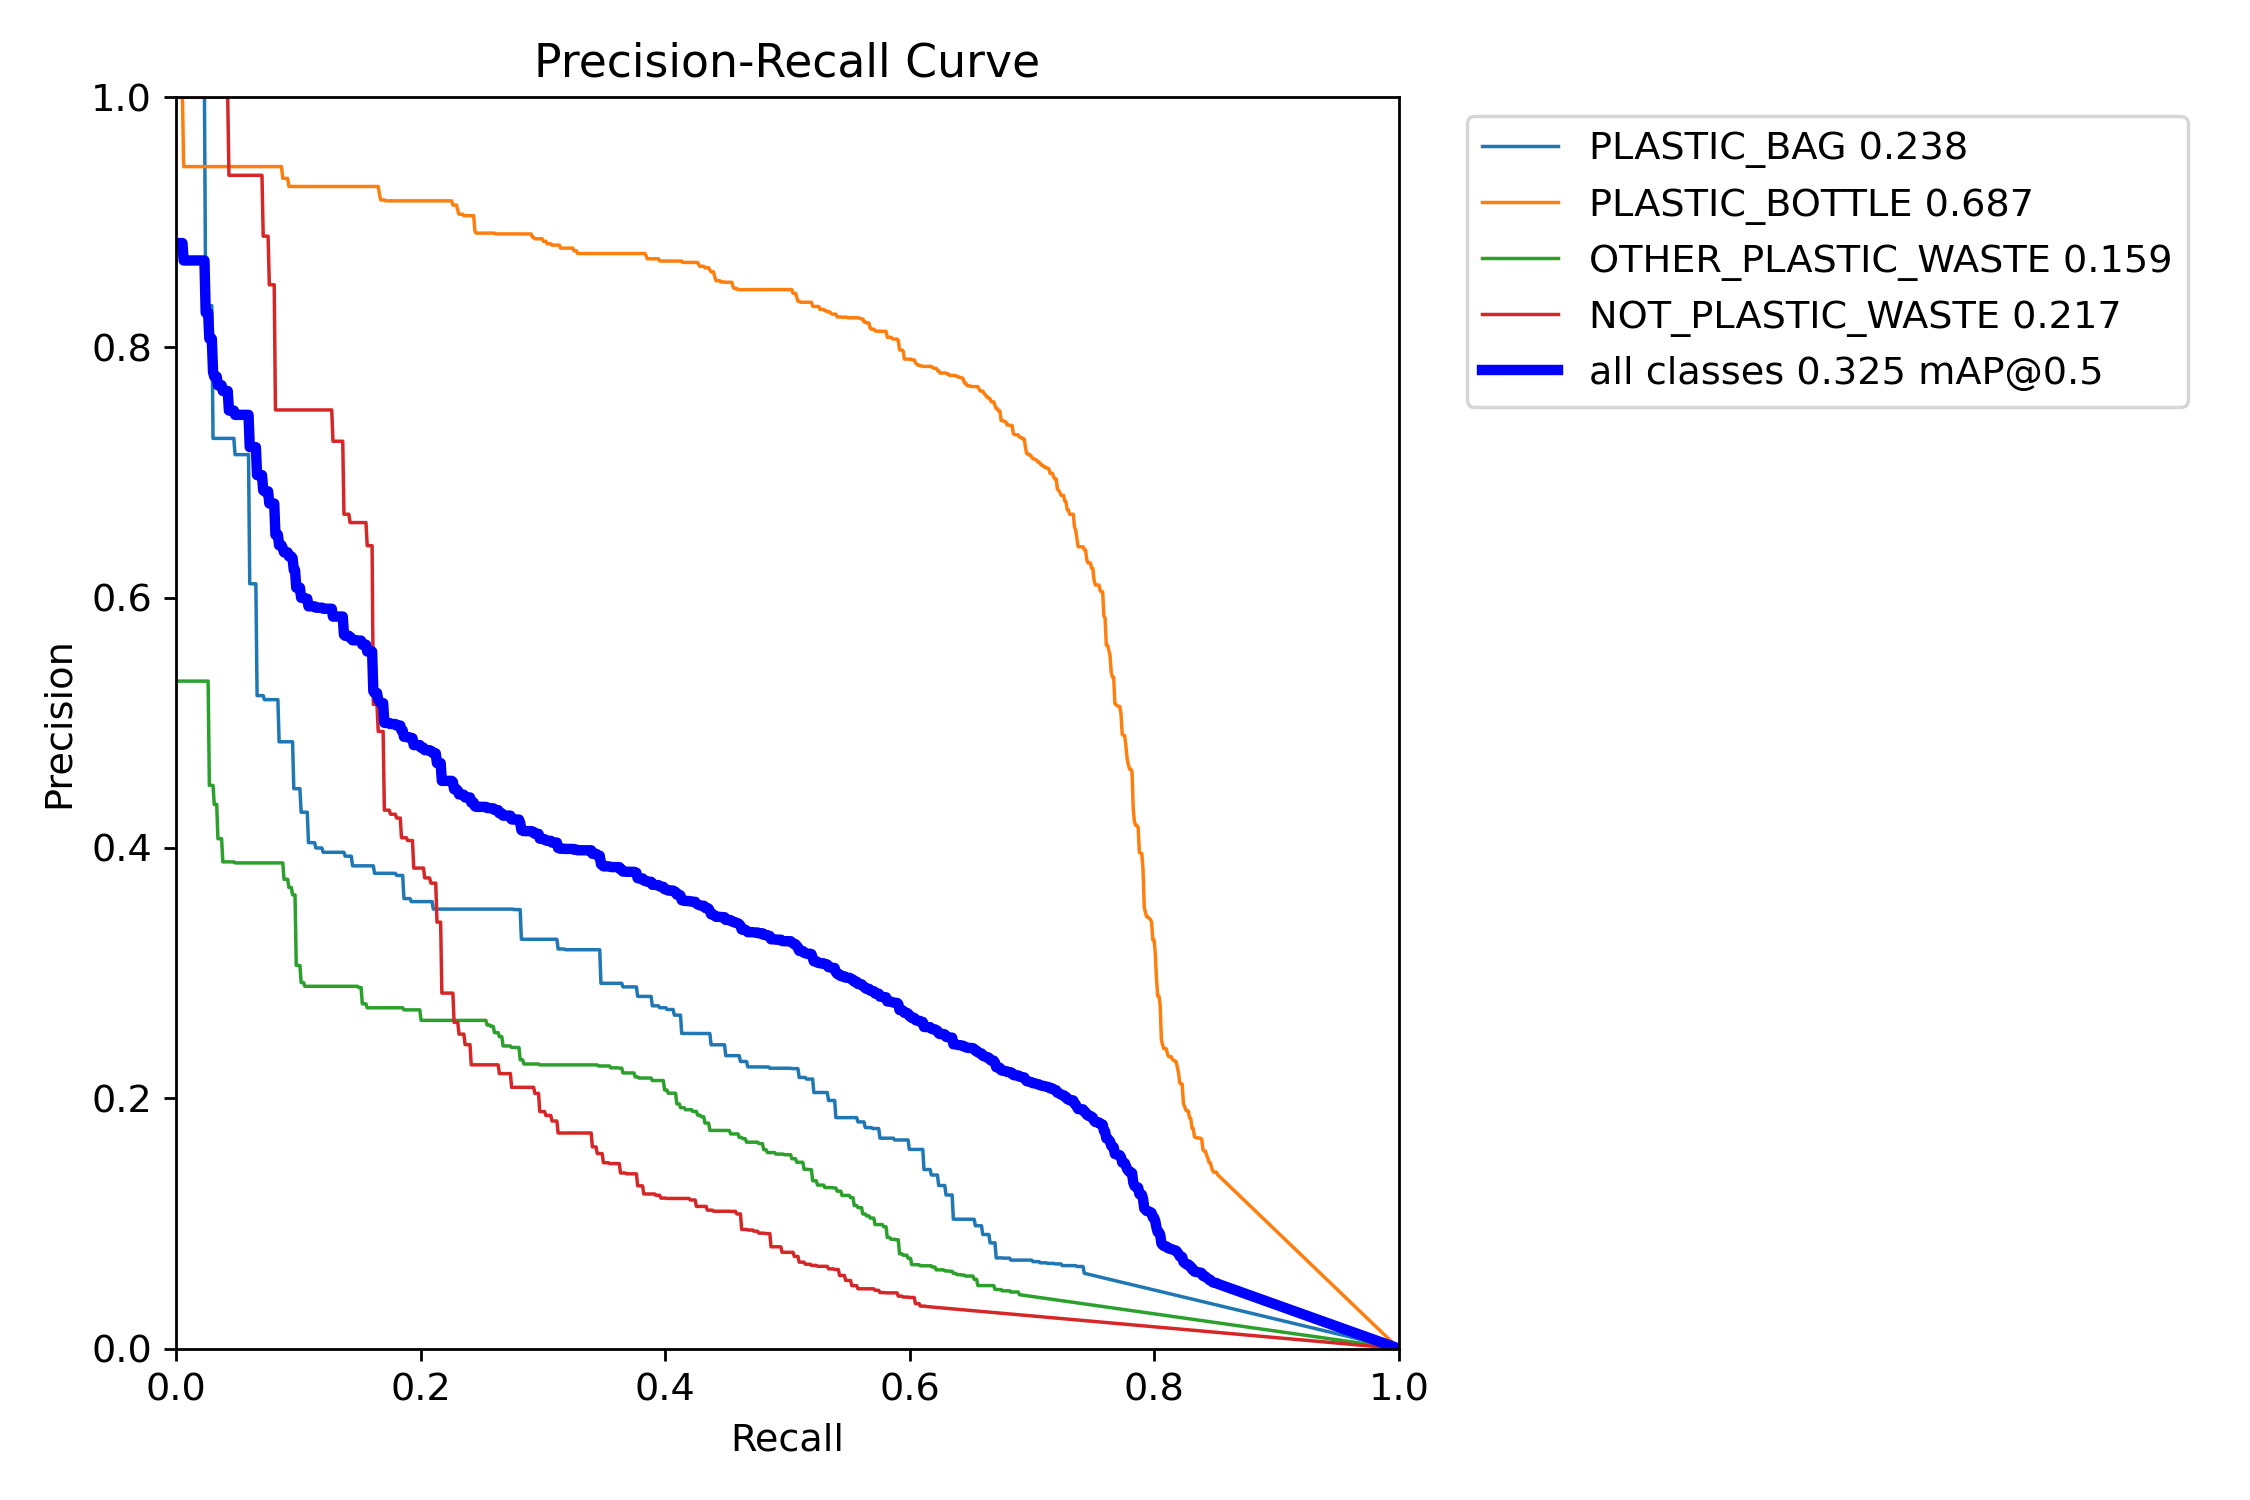
\includegraphics[width=.9\linewidth]{v_2/small-1203/PR_curve.png}
          \label{fig:v2-3.3}
        \end{subfigure}
        \begin{subfigure}{.49\textwidth}
            \centering
            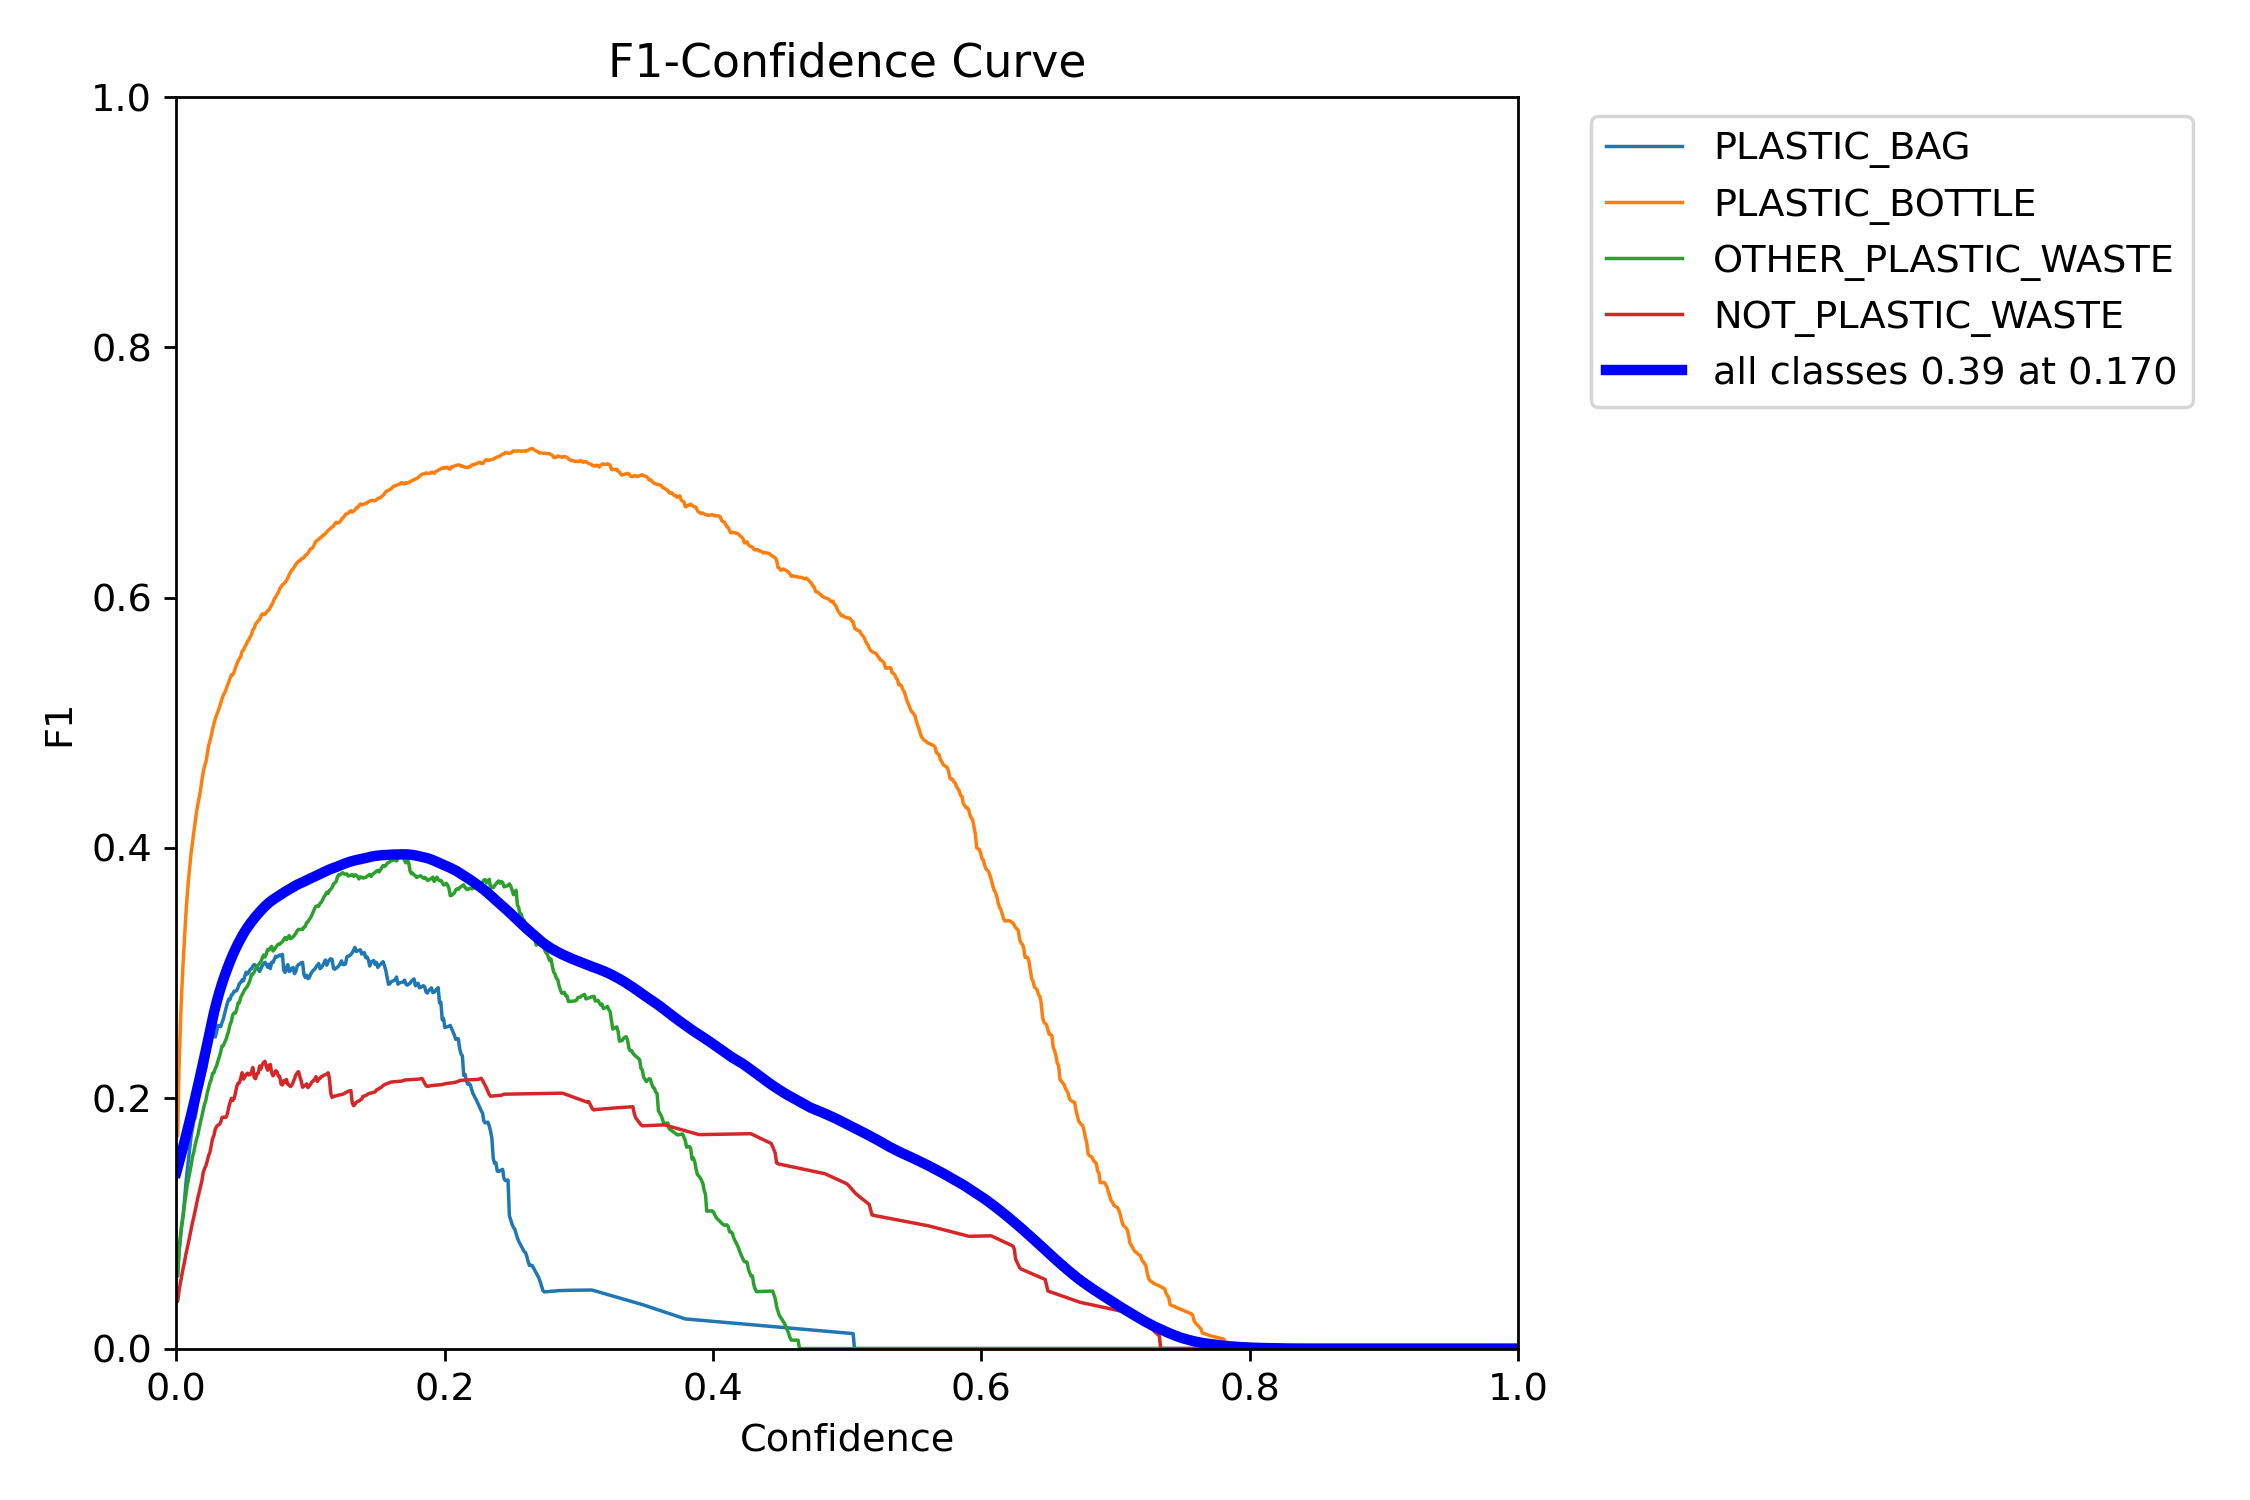
\includegraphics[width=.9\linewidth]{v_2/small-1203/F1_curve.png}
            \label{fig:v2-3.4}
          \end{subfigure}

        \caption{Andamento funzioni di loss e metriche durante l'esecuzione di v8m12}
        \label{fig:v2-3}
    \end{figure}


    % - matrici di confusione
    
    % - tabella performance test set

% Commento risultati
Quello che si è potuto vedere dai risultati e dalle performance di questi modelli è che il modello
tende ad avere una discreta precisione e richiamo in generale ma non troppo soddisfacente. 
In particolare se si 

\newgeometry{left=1.5cm, right=1.5cm, top=2cm, bottom=2cm} % Modifica temporaneamente i margini
\begingroup
\small 

\begin{table}[h]
    \centering
    \begin{tabularx}{\textwidth}{lYYYYYY}
        \toprule
        Class & Images & Instances & Box(P & R & mAP50 & mAP50-95) \\
        \midrule
        ALL & 427 & 1172 & 0.452 & 0.450 & 0.374 & 0.172 \\
        PLASTIC\_BAG & 34 & 85 & 0.402 & 0.388 & 0.344 & 0.120 \\
        PLASTIC\_BOTTLE & 312 & 854 & 0.684 & 0.727 & 0.724 & 0.344 \\
        OTHER\_PLASTIC\_WASTE & 25 & 122 & 0.140 & 0.377 & 0.106 & 0.0367 \\
        NOT\_PLASTIC\_WASTE & 49 & 111 & 0.582 & 0.306 & 0.320 & 0.187 \\
        \bottomrule
    \end{tabularx}
    \caption{Risultati per \textit{small-1203}}
\end{table}

\endgroup % Fine della sezione ridotta
\restoregeometry % Ripristina i margini originali

\begin{figure}[h]
    \centering
    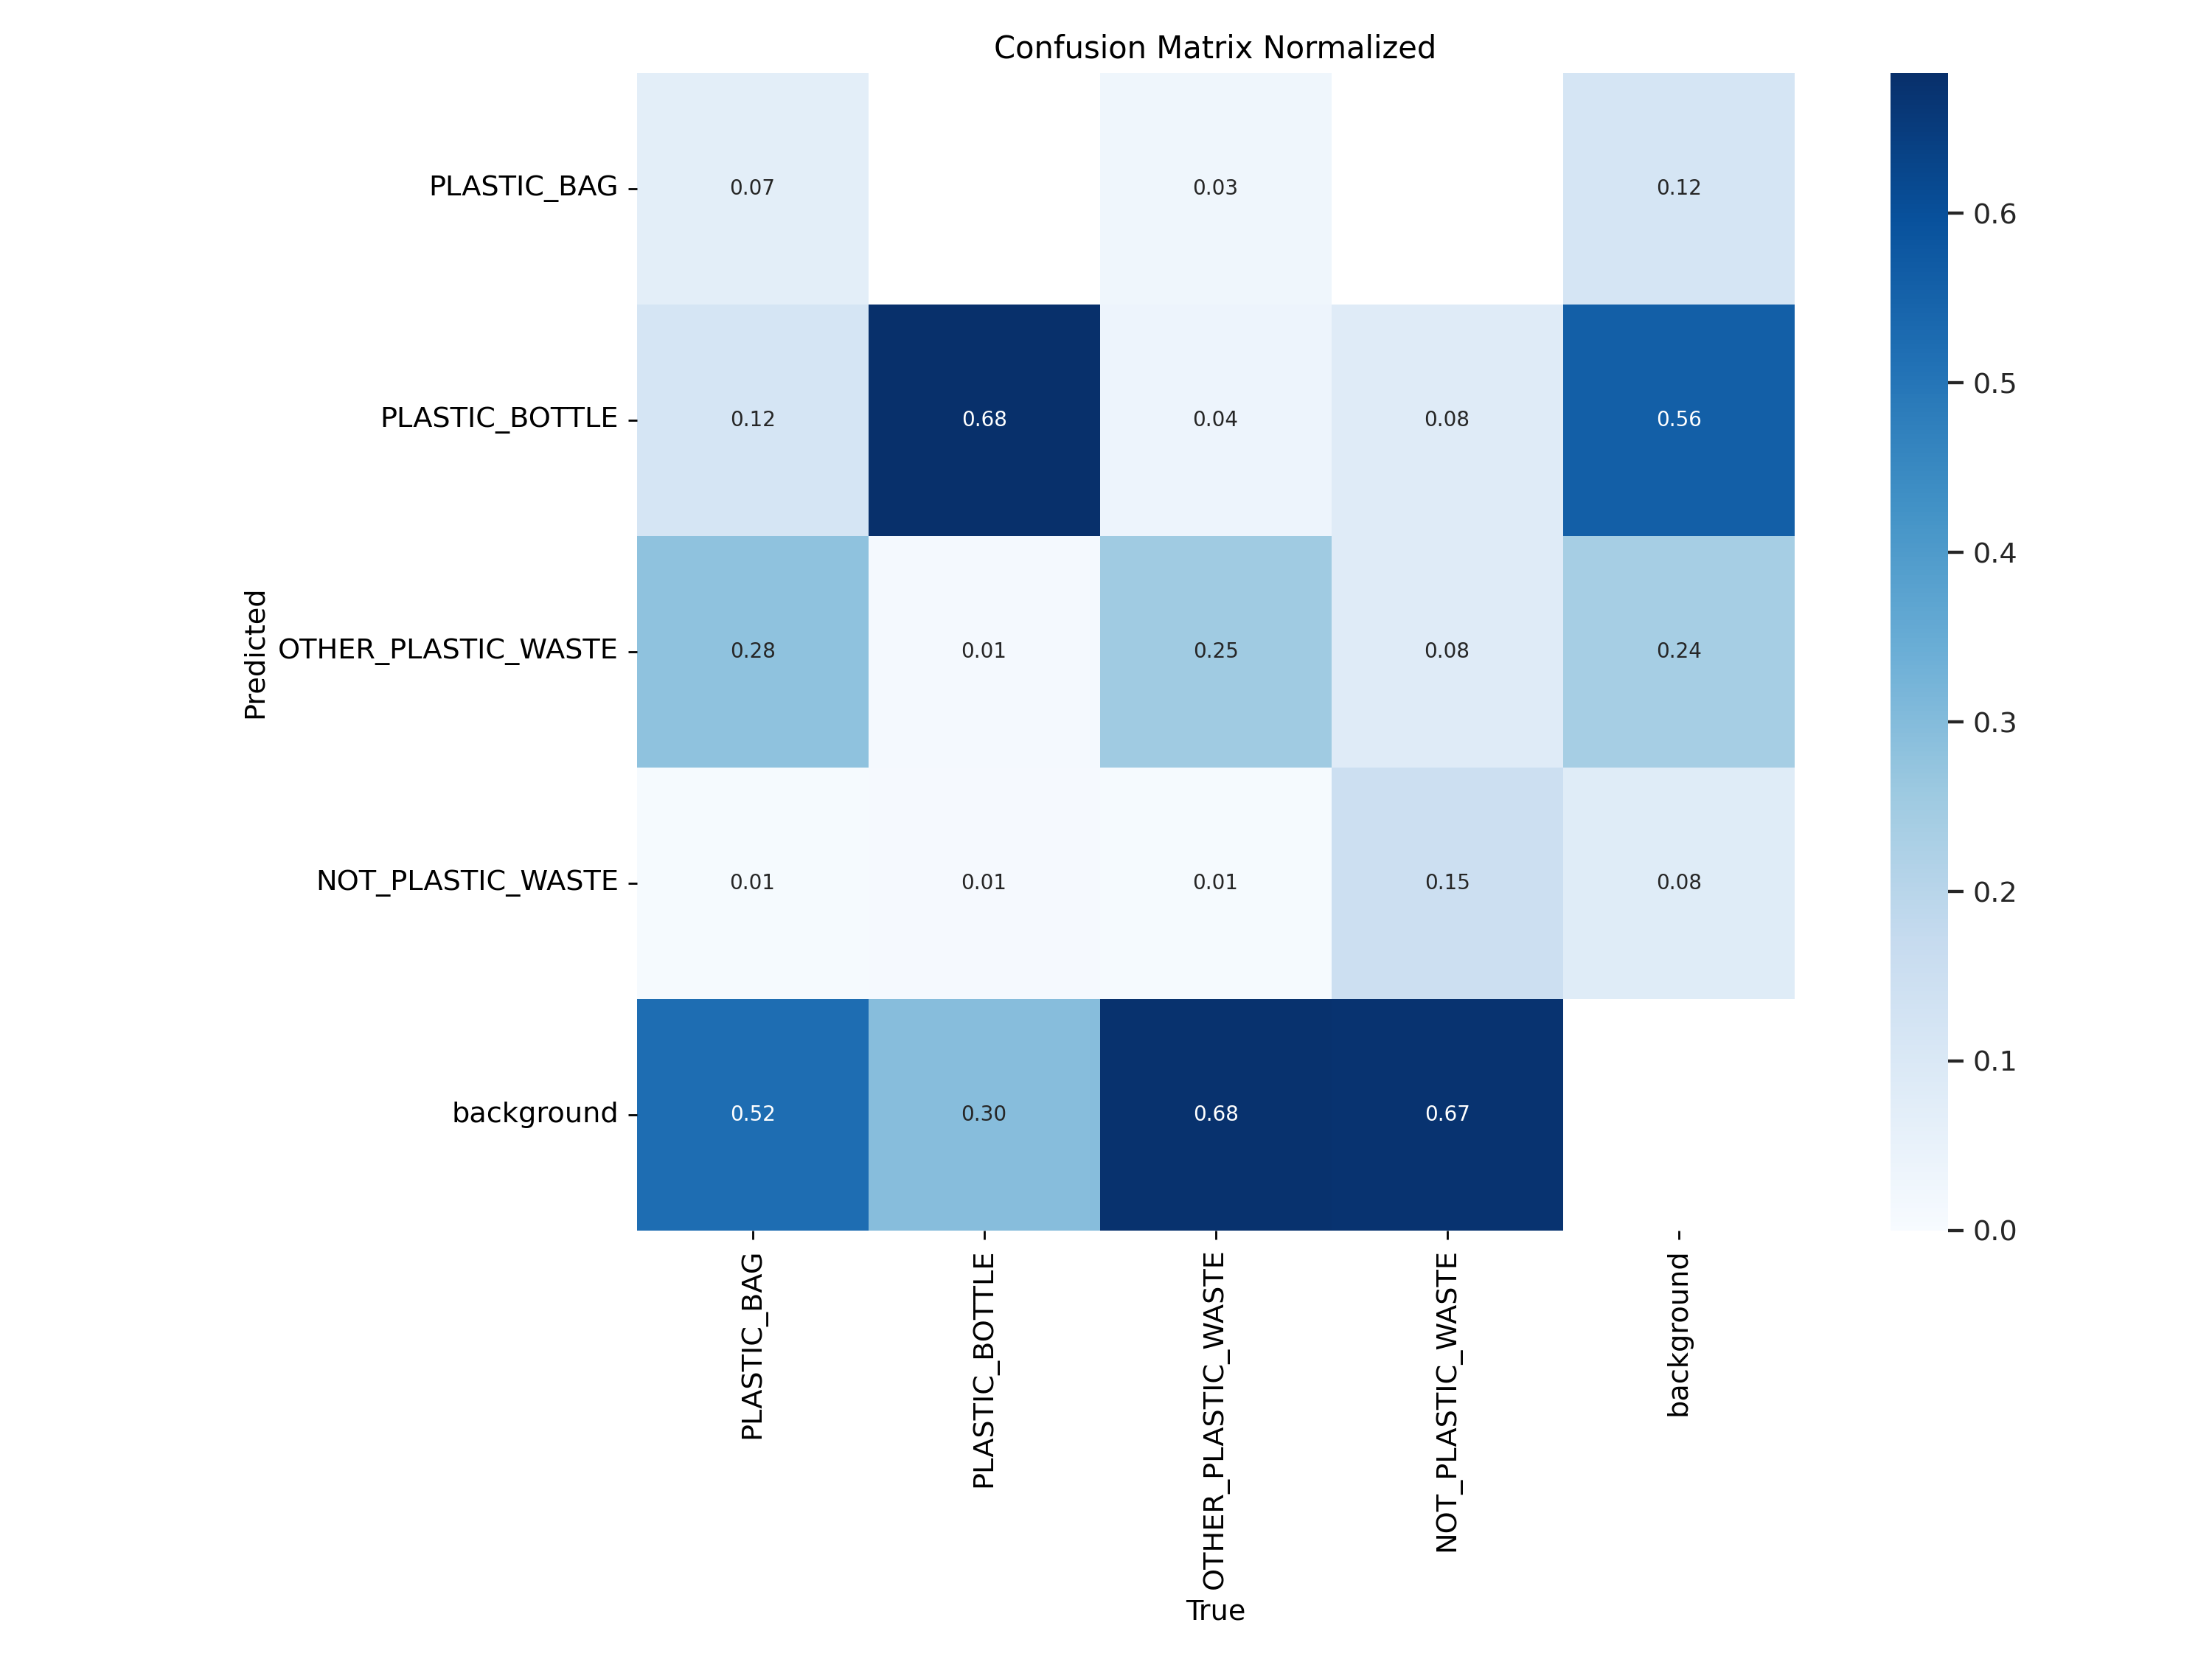
\includegraphics[width=0.8\textwidth]{v_2/small-1203/confusion_matrix_normalized.png}
    \caption{Matrice di confusione normalizzata data dal modello small-1203}
    \label{fig:v2-4}
\end{figure}